\documentclass[10pt]{article}
\usepackage[margin=0.60in]{geometry}
\usepackage{amsmath,booktabs,enumitem,fancyhdr,graphicx,listings,tabularx,titlesec,xcolor}
\usepackage[hidelinks]{hyperref}
\graphicspath{{docs/lessons/assets/}{../assets/}}
\hypersetup{
 pdftitle={ADK Lesson 061: Resistive-Probe Observations},
 pdfauthor={Kevin Shanahan},
 pdfsubject={Qualifying copied resistive-probe samples with calibration, excitation-off evidence, freshness, and bounded per-cycle duty},
 pdflang={en-US}}
\pagestyle{fancy}\fancyhf{}
\lhead{\textsc{ADK Lesson 061}}\rhead{Resistive-Probe Observations}
\cfoot{\thepage}\setlength{\headheight}{14pt}
\setlength{\parindent}{0pt}\setlength{\parskip}{3pt}
\setlist{nosep,leftmargin=1.45em}
\titleformat{\section}{\Large\bfseries}{\thesection}{0.5em}{}
\newcommand{\lessonbox}[1]{\begin{center}\fbox{\parbox{0.92\linewidth}{#1}}\end{center}}
\newcommand{\blankline}{\rule{0.76in}{0.4pt}}
\newcommand{\longblank}{\rule{1.35in}{0.4pt}}
\lstset{
 basicstyle=\ttfamily\footnotesize,
 columns=fullflexible,
 breaklines=true,
 frame=single,
 rulecolor=\color{black},
 showstringspaces=false}

\begin{document}
\small
\begin{center}
 {\Huge\bfseries Resistive-Probe Observations}\\[3pt]
 {\Large Decide what copied evidence supports---and what it cannot}\\[7pt]
 \fbox{\textbf{E0 SYNTHETIC REPLAY --- DO NOT WIRE OR ENERGIZE A PROBE}}
\end{center}
\begin{tabularx}{\linewidth}{@{}>{\bfseries}l X >{\bfseries}l X@{}}
Lesson & 061 --- component & Time & 150--210 minutes\\
Prerequisites & status, supplied time, copied evidence & Board & compile-only Mega replay\\
Input & one complete acquisition-cycle sample & Observation & named memory result cell\\
\end{tabularx}

\lessonbox{\textbf{Responsibility.}
\texttt{ResistiveProbeObservationPolicy} qualifies one copied conductive-probe
sample against fixed dry and wet references, explicit excitation evidence,
freshness, and a bounded per-cycle duty contract. It does not switch power,
read an ADC, identify a liquid, estimate depth, compensate contamination, or
prove that a physical leak is absent.}

\section{Start with an honest evidence boundary}
A conductive probe can produce an ADC-like number, but the number alone does
not explain the circuit that produced it. Geometry, ionic content,
contamination, corrosion, supply conditions, and acquisition timing can all
change the result. Lesson 061 therefore begins after acquisition: a synthetic
producer supplies a complete copied record, and a pure policy decides which
bounded interpretation that record supports.

\begin{center}
% ADK visual: pencil
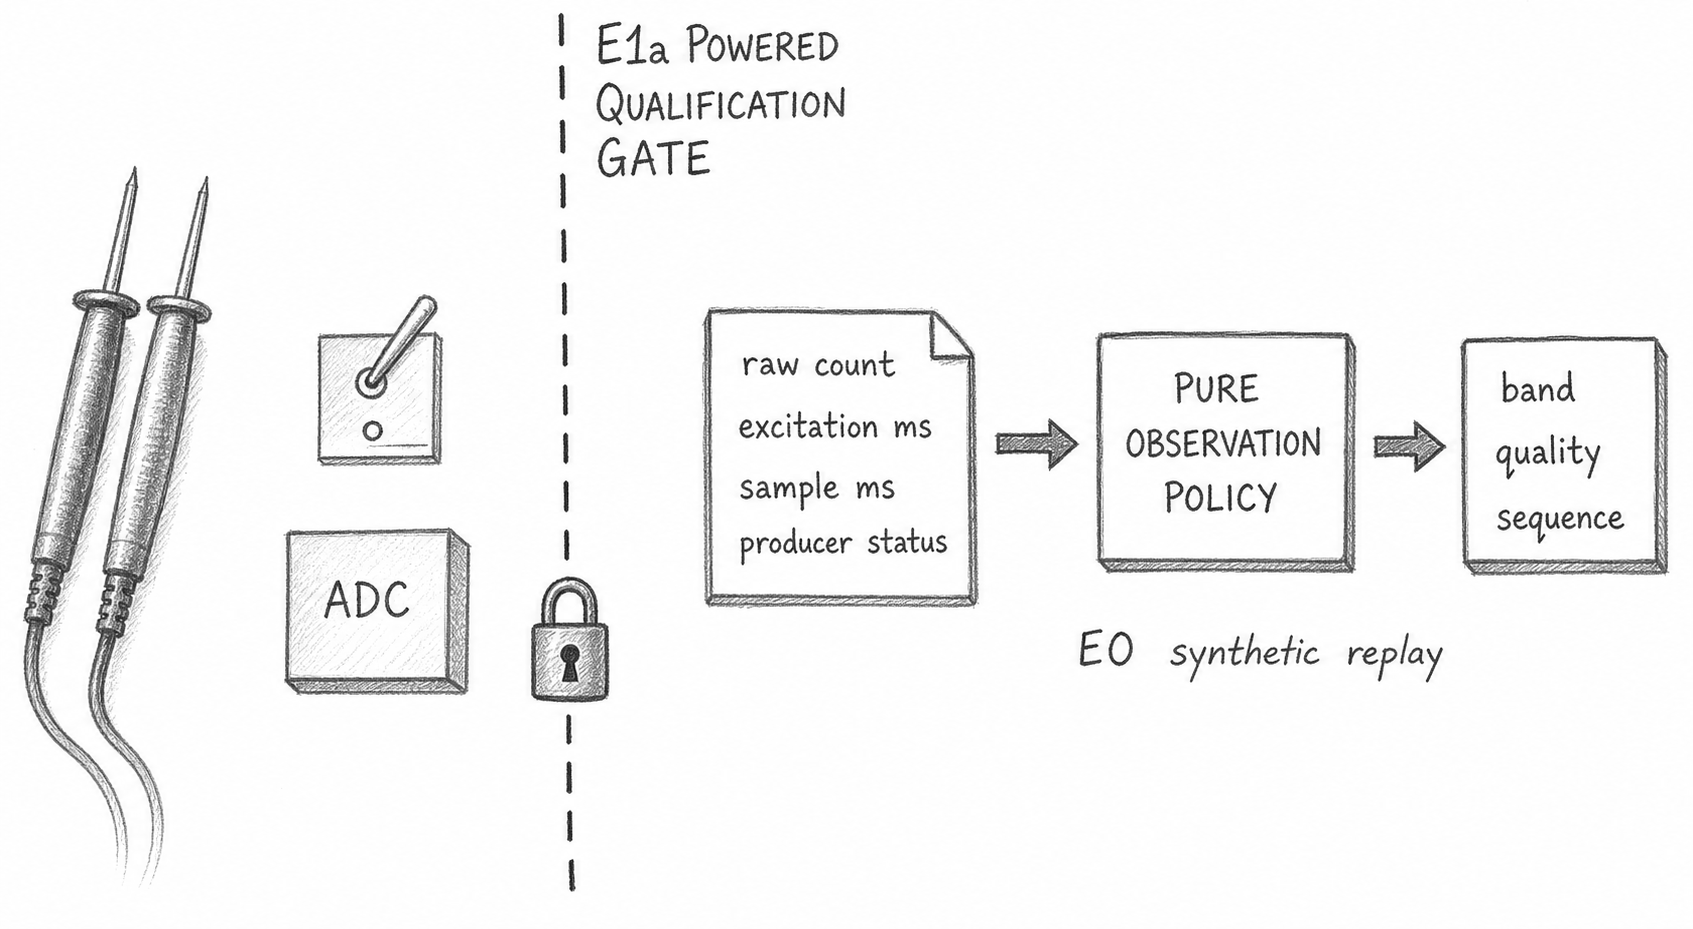
\includegraphics[width=0.94\linewidth,height=1.95in,keepaspectratio]
 {061-evidence-boundary-pencil.png}

\small\textit{Alternative text: a pencil-drawn boundary separates an
unqualified physical probe, excitation switch, and ADC on the left from a
copied sample card and pure observation policy on the right; a locked E1a gate
blocks every wire and powered claim.}
\end{center}

\begin{tabularx}{\linewidth}{@{}X X@{}}
\toprule
E0 proves & E0 does not prove\\
\midrule
deterministic classification of copied synthetic samples & an ADC channel or excitation pin was acquired\\
fixed calibration and threshold arithmetic & a kit probe has a particular topology or polarity\\
explicit off, timing, age, and provenance checks & excitation physically turned off\\
bounded volatile policy state & corrosion, current, spill, and drying safety\\
\bottomrule
\end{tabularx}

There is no formal electrical schematic in this lesson. An authoritative
schematic requires one exact specimen, its switched-excitation circuit, ADC
reference and source-impedance evidence, and measured safe-state behavior.
Those are E1a tasks, not blanks to fill with a generic module drawing.

\section{Copy one complete acquisition cycle}
The producer supplies the energized reading and the discharged reading from
the same named acquisition cycle. Identity and order travel with those
numbers: nonzero source, configuration, and calibration revisions; nonzero
producer sequence; observation time; producer status; on-time; cycle time;
and an explicit statement that excitation was observed off after sampling.

\begin{center}
% ADK visual: pencil
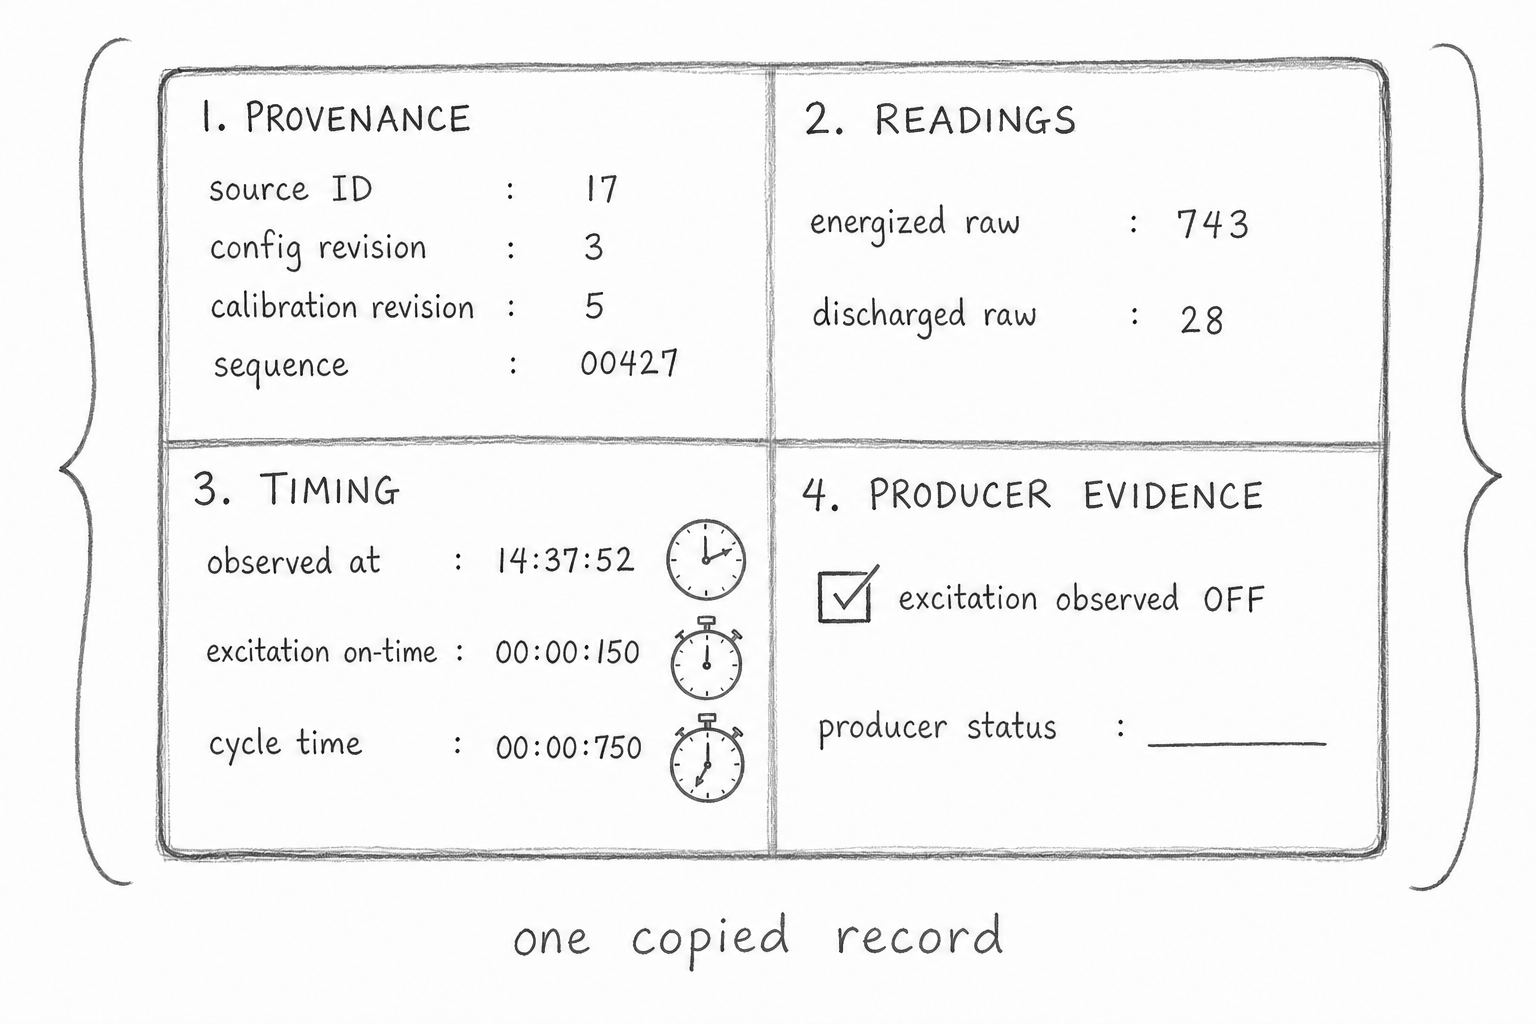
\includegraphics[width=0.96\linewidth,height=2.05in,keepaspectratio]
 {061-sample-card-pencil.png}

\small\textit{Alternative text: a hand-drawn sample card groups provenance,
energized and discharged readings, excitation on-time and cycle time, observed
off evidence, producer status, and observation time as one copied record.}
\end{center}

\begin{tabularx}{\linewidth}{@{}l X@{}}
\toprule
Field group & Question it makes answerable\\
\midrule
source and revisions & Which fixed producer and interpretation created this record?\\
sequence and time & Is it ordered, unambiguous, and fresh?\\
energized and discharged raw values & What happened during sampling and after excitation?\\
on-time and cycle time & What duty did this supplied cycle report?\\
off evidence and status & Did the producer observe cleanup, and did it report failure?\\
\bottomrule
\end{tabularx}

The policy copies the complete input and retains no caller pointer. Equal
timestamps are idempotent only for byte-identical duplicates. A changed
duplicate, backward time, exact modular half-range ambiguity, sequence
regression, or changed source/revision rejects atomically.

\section{Validate structure before interpreting liquid}
Configuration fixes the declared ADC maximum, dry and wet references,
disconnected and discharged limits, ordered damp and wet thresholds, maximum
age, maximum on-time, and maximum duty. The ADC maximum must be nonzero. All
raw values, calibration references, and disconnected and discharged limits
must fit its declared domain. Dry and wet references must differ, while either
slope is allowed.

\begin{center}
% ADK visual: pencil
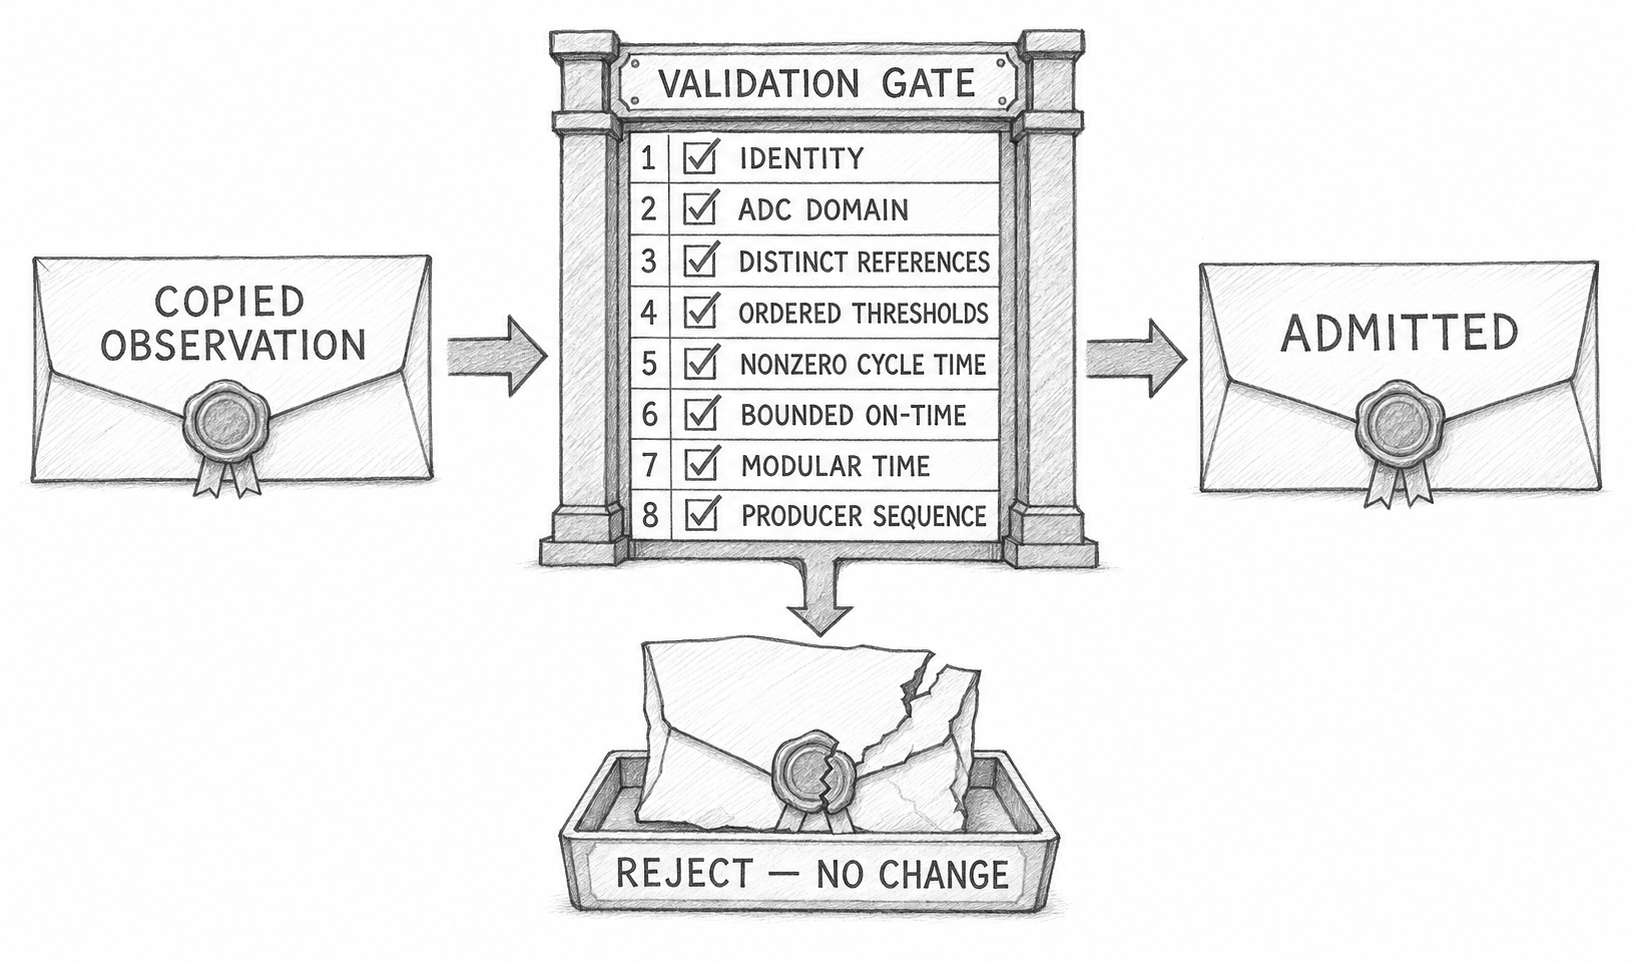
\includegraphics[width=0.95\linewidth,height=1.90in,keepaspectratio]
 {061-validation-gate-pencil.png}

\small\textit{Alternative text: pencil checkpoints inspect identity, ADC
domain, distinct references, ordered thresholds, nonzero cycle time, bounded
on-time, modular time, and producer sequence before a sealed observation card
is allowed to change.}
\end{center}

\begin{enumerate}
 \item Check lifecycle, fixed configuration, source identity, revisions,
       sequence, and modular time.
 \item Check raw values and references against the declared ADC domain.
 \item Require nonzero cycle time and on-time no greater than cycle time.
 \item Compute duty with widened arithmetic so
       \texttt{onTime * 1000 / cycleTime} cannot overflow.
 \item Only after structural admission, apply the quality precedence.
\end{enumerate}

Predict the result when a malformed cycle also contains a convincingly wet
energized value: \longblank. Explain why interpretation cannot precede
structure: \longblank.

\section{Normalize either calibration slope}
Normalization maps the dry reference to 0 permille and the wet reference to
1000 permille. Values between them are monotonic. Values beyond either
reference clamp to the nearest endpoint for ordinary classification. The
arithmetic must work whether wet is numerically above or below dry.

\begin{center}
% ADK visual: pencil
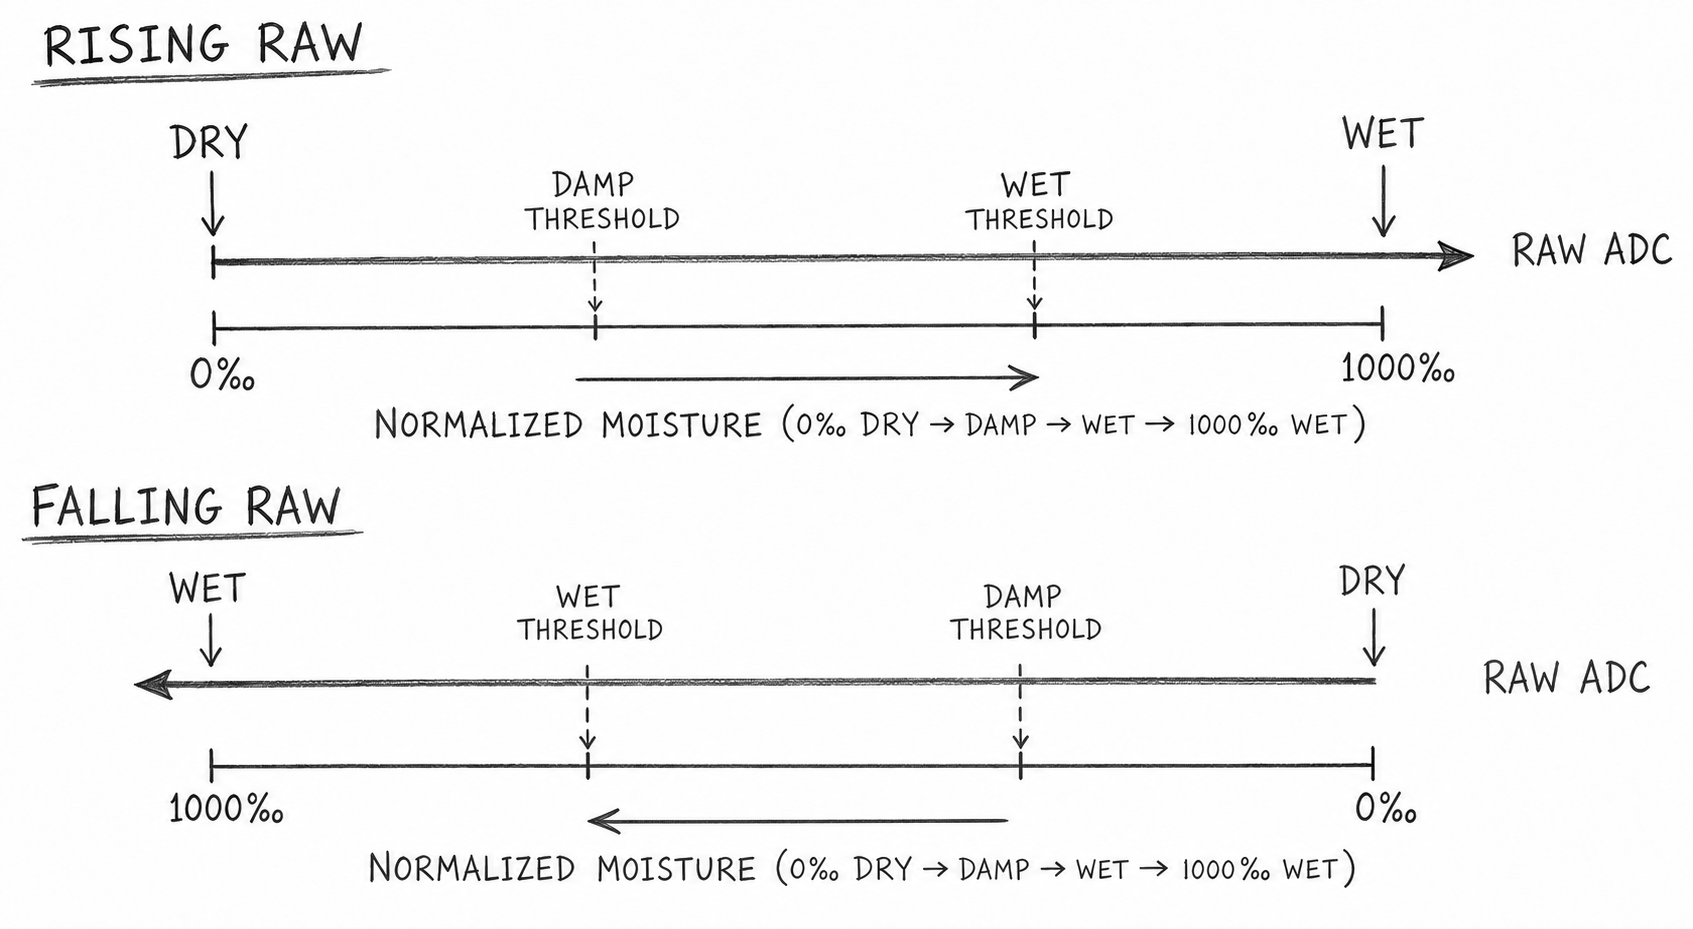
\includegraphics[width=0.95\linewidth,height=2.05in,keepaspectratio]
 {061-calibration-slopes-pencil.png}

\small\textit{Alternative text: two pencil number lines show rising and
falling calibrations; both map their dry reference to zero permille and wet
reference to one thousand, with the damp and wet thresholds crossed in the
same normalized order.}
\end{center}

\begin{tabularx}{\linewidth}{@{}l l l@{}}
\toprule
Normalized value & Threshold relationship & Ordinary quality\\
\midrule
below damp threshold & dry side of both thresholds & \texttt{Dry}\\
at or above damp, below wet & between ordered thresholds & \texttt{Damp}\\
at or above wet & wet side of both thresholds & \texttt{Wet}\\
\bottomrule
\end{tabularx}

Fill one rising calibration with dry \(=200\), wet \(=800\). What normalized
value should raw \(=500\) produce? \blankline\ permille. Reverse the
references. What should raw \(=500\) produce now? \blankline\ permille.

Threshold tests inspect immediately below, exactly at, and immediately above
each boundary. Integer arithmetic defines these boundaries; a replay must not
depend on floating-point rounding.

\section{Give faults precedence over an attractive number}
A valid update applies a fixed order. Producer failure precedes every domain
quality. Missing off evidence, excessive discharged reading, excessive
on-time, or excessive duty produces \texttt{ExcitationFault}. Exact ADC
full-scale energized input produces \texttt{Saturated}. The deliberately
narrow disconnected predicate requires \emph{both} energized and discharged
values at or below the disconnected maximum.

\begin{center}
% ADK visual: pencil
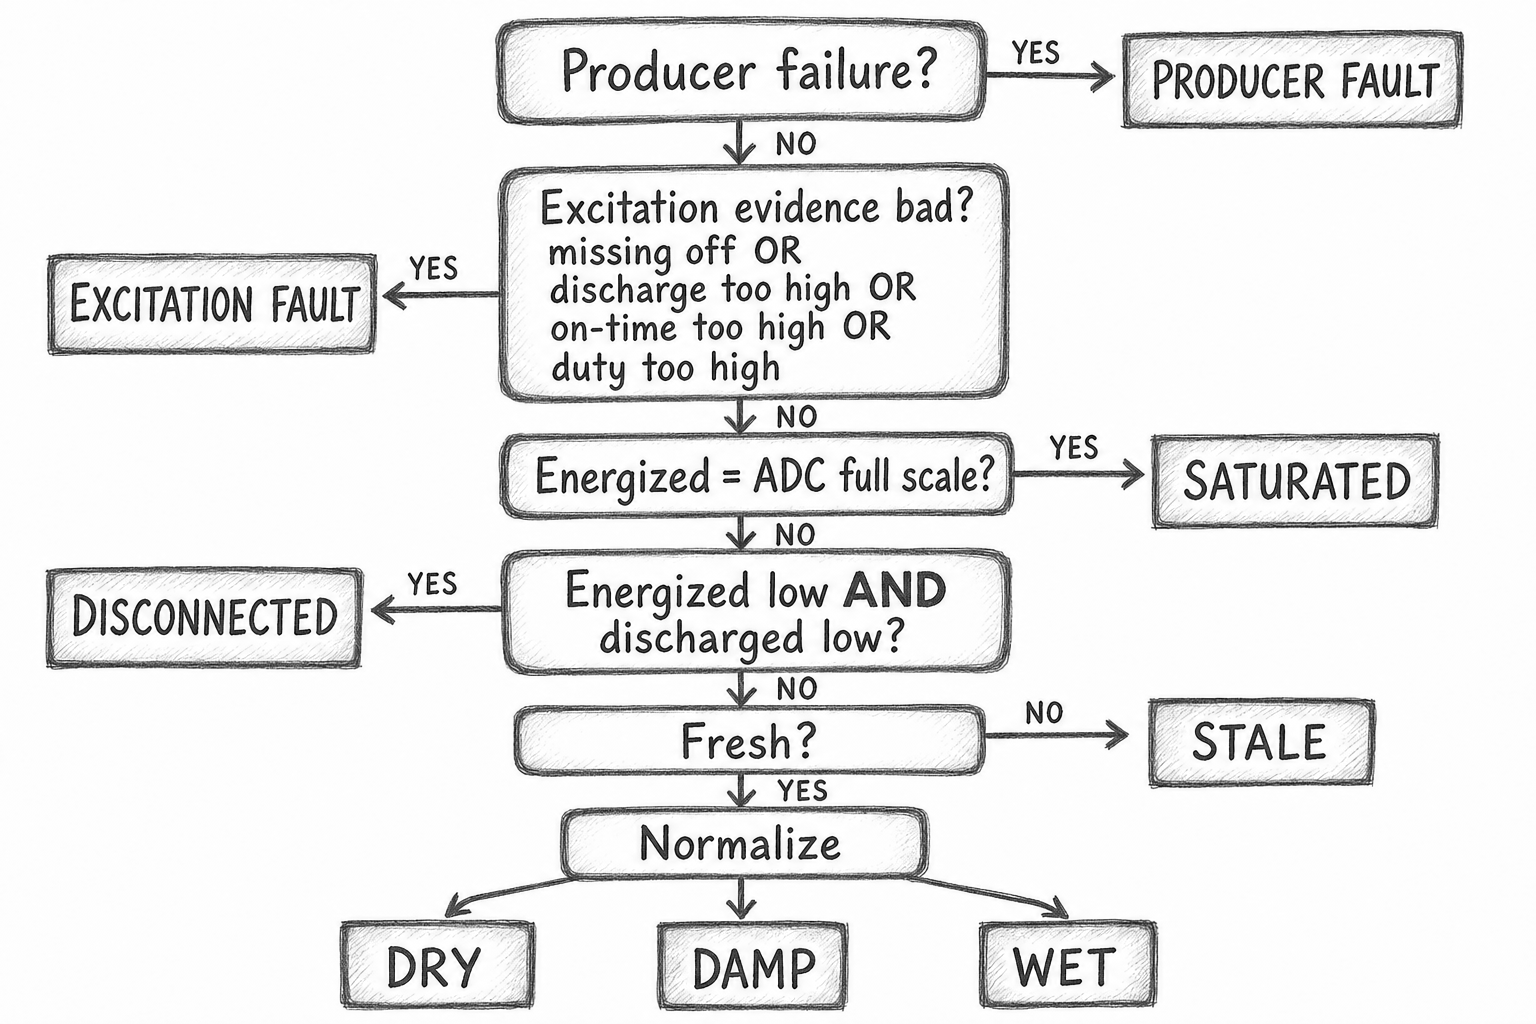
\includegraphics[width=0.96\linewidth,height=2.25in,keepaspectratio]
 {061-quality-precedence-pencil.png}

\small\textit{Alternative text: a pencil decision path checks producer
failure, excitation and discharge evidence, exact full-scale saturation, the
two-low-values disconnected predicate, freshness, and only then normalized
dry, damp, or wet classification.}
\end{center}

\begin{tabularx}{\linewidth}{@{}l X l@{}}
\toprule
Evidence & Why it dominates & Quality\\
\midrule
producer reports failure & sample meaning is not trustworthy & \texttt{ProducerFault}\\
off missing or discharge/on-time/duty excessive & cleanup contract failed & \texttt{ExcitationFault}\\
energized raw equals ADC maximum & rail cannot be relabeled ``very wet'' & \texttt{Saturated}\\
both raw values at or below disconnected maximum & exact qualified synthetic predicate & \texttt{Disconnected}\\
age exceeds maximum & otherwise valid evidence arrived too late & \texttt{Stale}\\
all earlier checks pass & calibrated thresholds may be interpreted & dry/damp/wet\\
\bottomrule
\end{tabularx}

An arbitrary open circuit need not read low, and arbitrary contamination need
not resemble the calibration fixture. The disconnected rule is a fixed
synthetic contract awaiting E1 qualification, not a universal electrical
diagnosis. Likewise, \texttt{Dry} means only ``classified on the dry side of
this fixed calibration''; it never certifies that a case has no leak.

\section{Measure only the supplied cycle's duty}
For one admitted sample, observed cycle duty is
\[
 \left\lfloor
 \frac{\text{excitation on-time}\times 1000}{\text{cycle time}}
 \right\rfloor .
\]
The policy checks this value and the independent maximum on-time. It retains
no rolling energy history, so it cannot prove cumulative energized time,
long-term corrosion duty, or compliance between supplied samples.

\begin{center}
% ADK visual: pencil
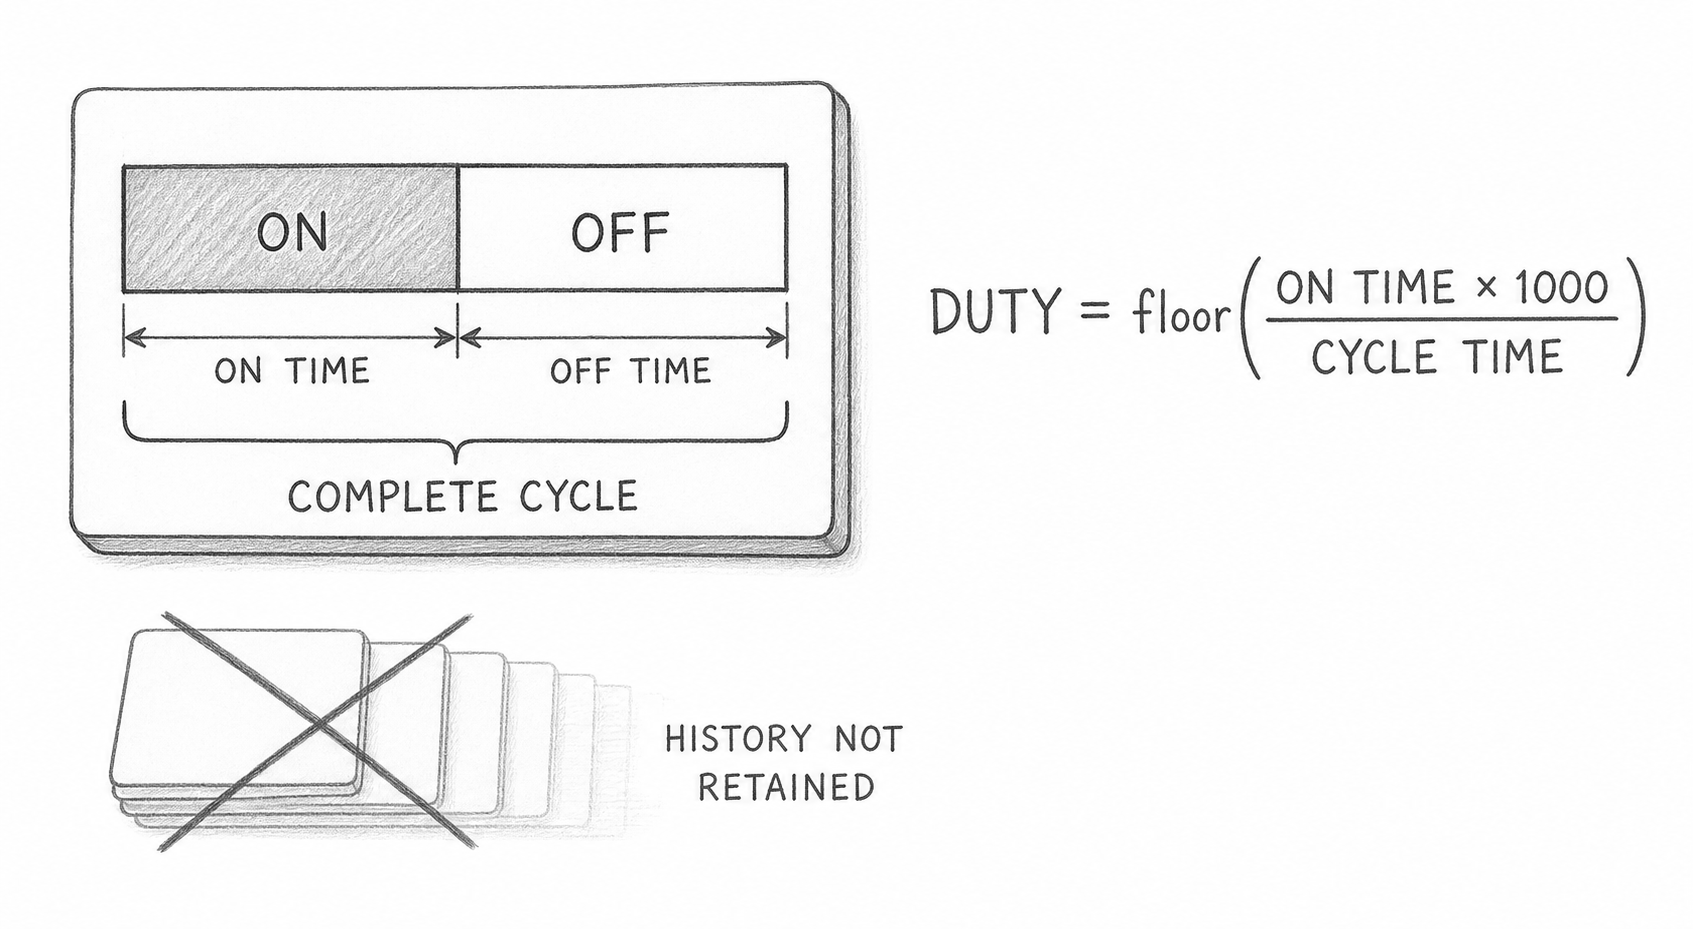
\includegraphics[width=0.94\linewidth,height=1.90in,keepaspectratio]
 {061-duty-window-pencil.png}

\small\textit{Alternative text: a pencil timing strip shows one bounded cycle
with a short shaded excitation interval and a longer discharged interval; a
bracket labels per-cycle duty while a broken line beyond the cycle is marked
unknown history.}
\end{center}

\begin{tabularx}{\linewidth}{@{}l l l X@{}}
\toprule
On-time & Cycle time & Duty & Interpretation\\
\midrule
0 & 100 ms & 0 permille & no reported excitation in this cycle\\
5 ms & 100 ms & 50 permille & supplied-cycle result only\\
100 ms & 100 ms & 1000 permille & continuously on for this cycle\\
101 ms & 100 ms & invalid & structural rejection before division\\
\bottomrule
\end{tabularx}

For 7 ms on during a 64 ms cycle, predict the truncated duty:
\blankline\ permille. Then name the evidence still needed to make a physical
corrosion-duty claim: \longblank.

\section{Make age and ordering deterministic}
\texttt{TimePoint now} is the only clock. Age is derived with modular unsigned
time rules; every configured duration remains strictly below the half range.
Evidence at exactly the maximum age is admitted. Evidence one tick older is
\texttt{Stale}. Backward time and exact half-range ambiguity reject without
changing the last accepted observation.

\begin{center}
% ADK visual: pencil
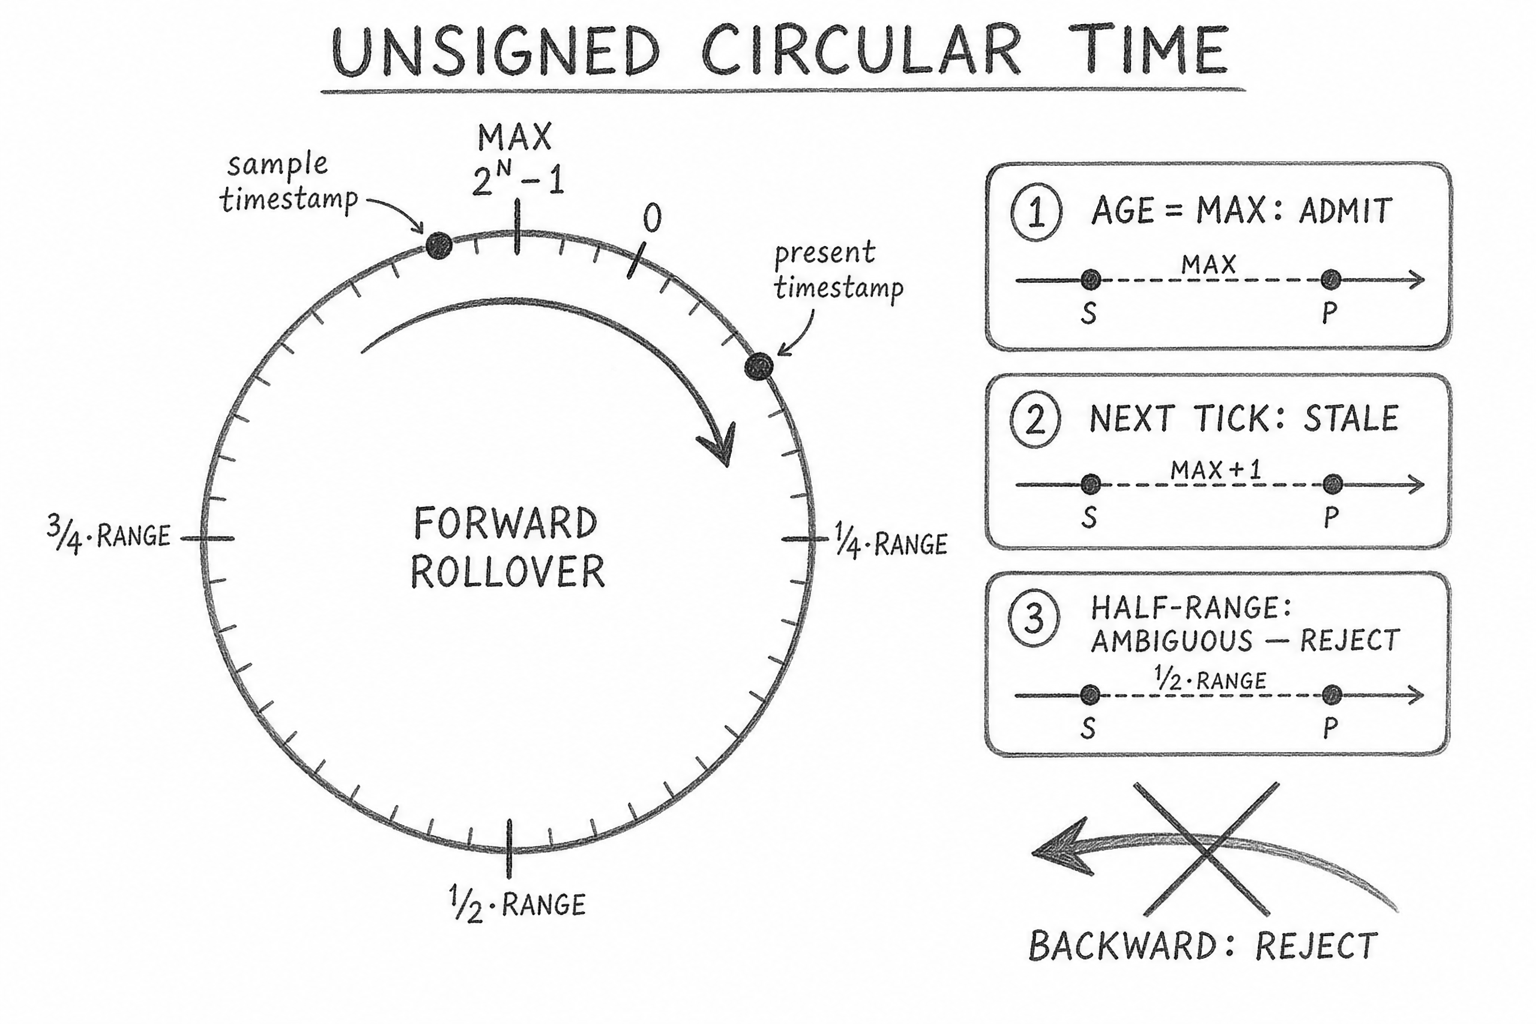
\includegraphics[width=0.95\linewidth,height=1.85in,keepaspectratio]
 {061-freshness-rollover-pencil.png}

\small\textit{Alternative text: a hand-drawn circular counter crosses
unsigned rollover from a late observation to a small current time; tick marks
show the inclusive maximum-age boundary, the first stale tick, and a forbidden
half-range chord.}
\end{center}

Replay these cases before running tests:
\begin{enumerate}
 \item an otherwise-dry observation at the inclusive age limit:
       stale or admitted? \blankline;
 \item same timestamp and sequence with byte-identical content:
       disposition \blankline;
 \item same timestamp and sequence with one changed raw value:
       disposition \blankline;
 \item sequence \texttt{0xFFFFFFFE} followed by
       \texttt{0xFFFFFFFF} across ordinary clock rollover:
       accepted or rejected? \blankline;
 \item after accepting \texttt{0xFFFFFFFF}, attempt a duplicate and then
       sequence 1: what status must both return? \longblank;
 \item after explicit reset, attempt sequence 1:
       accepted or rejected? \blankline;
 \item an exact half-range time difference:
       accepted or rejected as ambiguous? \blankline.
\end{enumerate}

Sequence zero is always invalid. Accepting \texttt{UINT32\_MAX} latches
sequence exhaustion: every later update, including a duplicate, returns
\texttt{CapacityExceeded} atomically. Only explicit reset clears the latch
and begins a new volatile sequence epoch. This is bounded ordering behavior,
not durable producer identity across a restart.

\section{Replay the policy without hardware}
The Mega sketch constructs copied samples and writes observations to a named
result cell. It does not read a pin, energize a probe, acquire a timer, or
claim a visible physical result. The HTML lesson is the hardware-independent
route to the same learning outcome.

\begin{lstlisting}
ResistiveProbeObservationPolicy probe(config);
probe.initialize();

sample.sequence += 1U;
sample.observedAt = now;
const Status updateStatus = probe.update(now, sample);
const ResistiveProbeObservation result = probe.snapshot();
\end{lstlisting}

\begin{center}
% ADK visual: pencil
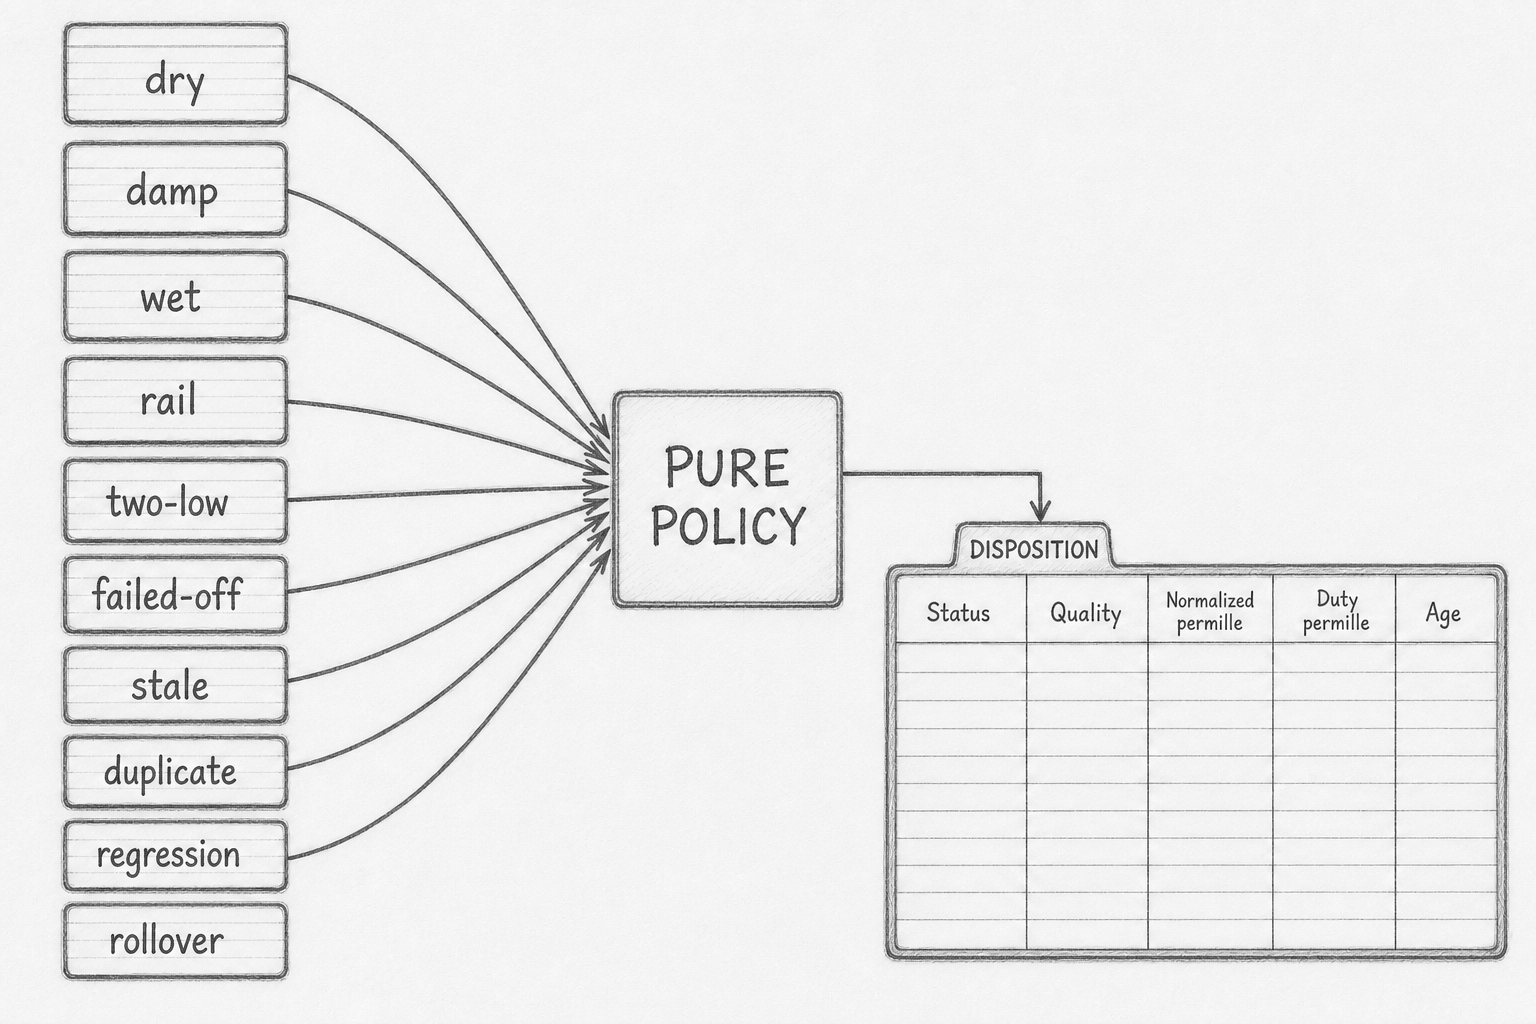
\includegraphics[width=0.94\linewidth,height=1.95in,keepaspectratio]
 {061-replay-ledger-pencil.png}

\small\textit{Alternative text: a pencil replay ledger feeds dry, damp, wet,
rail, two-low, failed-off, stale, duplicate, regression, and rollover sample
cards into one policy and records status, quality, normalized value, duty, and
age in named result cells.}
\end{center}

The deterministic proof covers both calibration slopes; ADC endpoints;
references and thresholds below, at, and above boundaries; dry-to-wet and
contamination-drift ramps; open, rail, stuck, incomplete-discharge, backfeed,
duty, stale, producer-fault, duplicate, regression, rollover, reset, and
byte-stable replay traces.

The canonical replay also records the reset snapshot and initialization
status, then admits a fresh sequence after reset. Reset clears the observation
and ordering history while preserving the validated configuration and
initialized lifecycle; a repeated \texttt{initialize()} is idempotent. The
named cells establish only that volatile policy transition.

\section{Inspect evidence before making a claim}
\begin{tabularx}{\linewidth}{@{}l X X@{}}
\toprule
Gate & Pass evidence & A pass still does not establish\\
\midrule
resource acquisition & zero pins, ADC channels, timers, buses, endpoints, or supplies & powered circuit availability\\
safe state & pure reset and rejected updates preserve bounded policy state & physical excitation removal\\
classification & exact precedence and golden normalized values & liquid identity or depth\\
time/order & age, duplicate, regression, and rollover traces & sampling cadence between records\\
replay & byte-identical result ledger & bench repeatability\\
\bottomrule
\end{tabularx}

The canonical measurements are 5,662 bytes of flash and 624 bytes of static
SRAM for the ordinary Mega replay, and 3,566 bytes of flash plus 169 bytes of
static SRAM for the isolated no-LTO probe. The conservative synchronous stack
is 123 bytes; the policy object is 69 bytes; and caller-owned input and output
buffers are 27 and 37 bytes, or 64 bytes together. After the specified
128-byte ISR reserve, 7,772 bytes of Mega SRAM remain after static SRAM and
the synchronous stack.

The ordinary sketch and isolated no-LTO probe are distinct measurement
boundaries; their flash and static-SRAM figures are not one aggregate. The
gate also checks ABI/ownership, retained-return stack edges, and the toolchain
fingerprint. These compiler results do not substitute for electrical or
physical evidence.

\lessonbox{\textbf{E1a remains open.}
Before any powered adapter, wiring, schematic, or support claim, qualify one
exact probe and circuit: switched excitation, ADC reference and source
impedance, off/backfeed behavior, current, duty waveform over the complete
campaign, corrosion, spill containment, drying, calibration stability, and a
non-Serial physical observation path.}

\section{Completion record}
Record the exact evidence you inspected.

\begin{tabularx}{\linewidth}{@{}X X@{}}
\toprule
Check & Result or evidence\\
\midrule
Both calibration slopes and threshold neighbors & \\
\addlinespace[1.2em]
Excitation-off, discharge, on-time, and duty precedence & \\
\addlinespace[1.2em]
Saturation and exact two-low disconnected predicate & \\
\addlinespace[1.2em]
Fresh/stale boundary, duplicate, regression, and rollover & \\
\addlinespace[1.2em]
Reset, replay determinism, and named result cell & \\
\addlinespace[1.2em]
Canonical numeric resource report and all hard gates & \\
\addlinespace[1.2em]
Zero-hardware E0 boundary and open E1a work & \\
\addlinespace[1.2em]
\bottomrule
\end{tabularx}

\begin{center}
\fbox{\parbox{0.90\linewidth}{
\textbf{Completion statement:} I can distinguish copied acquisition evidence
from physical qualification, apply structural and quality precedence,
normalize either calibration slope, explain the narrow disconnected predicate
and per-cycle duty limit, and identify every powered claim that remains open.

\vspace{0.10in}
Learner: \longblank\quad Reviewer: \longblank\quad Date: \blankline
}}
\end{center}

This print edition is untagged. Its text is searchable and copyable, and the
HTML lesson provides the hardware-independent alternative. No PDF/UA, WCAG,
or other PDF accessibility-conformance claim is made.

\end{document}
